\chapter{Beispielanwendung von Spark zur Datenanalyse}

Zur vertiefenden Betrachtung von Spark wird im Folgenden die Implementation einer Beispielanwendung gezeigt.\\

Dazu sollen mindestens zwei verschiedene Standardbibliotheken und deren Integration in eine gemeinsame Anwendung durchgeführt werden.\\

Anschließend werden rudimentäre Skalierungs- und Stresstests der Anwendung durchgeführt und der durchgeführte Versuch unter den Kriterien \textit{Einfachheit}, \textit{Skalierbarkeit}, \textit{Erweiterbarkeit}, \textit{Robustheit}, \textit{Sicherheit} und \textit{Wartbarkeit} zusammengefasst und bewertet.

\section{Vorstellung des Anwendungsfalls}
In dem Anwendungsfall soll ein Dashboard erstellt werden, auf dem Textnachrichten angezeigt werden.
Die Textnachrichten werden aus einem Datenstrom gelesen und dabei - entsprechend ihrer aktuellen Relevanz für einen Sparkbenutzer - bewertet und gefiltert. Als Maßstab für die Relevanz sollen Begriffen dienen, die kürzlich in der Mailingliste der Sparkbenutzer diskutiert wurden.\\

\begin{figure}[ht!]
	\centering
  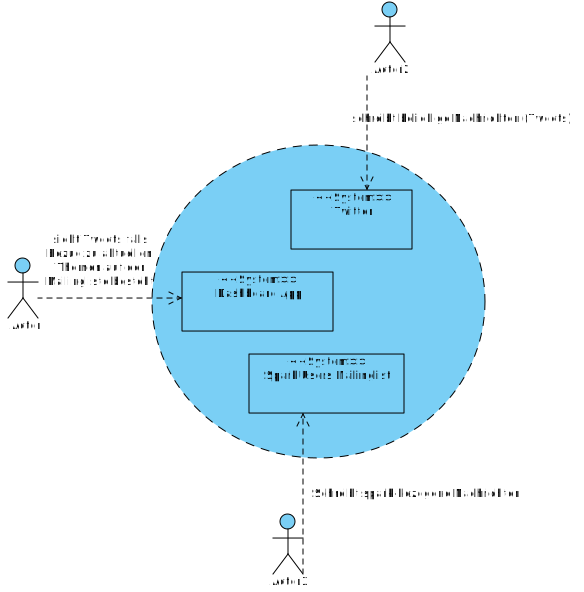
\includegraphics[scale=0.7]{demo_app_usecase.pdf}
	\caption{Anwendungsfalldiagramm der Demo-Applikation}
	\label{figure:demo_app_usecase}
\end{figure}

Als Datenquellen dienen einerseits die Emails aus der Malingliste\footnote{user@spark.apache.org} und andererseits der öffentliche Datenstrom\footnote{https://dev.twitter.com/streaming/sitestreams} mit Textnachrichten (\glspl{tweet}) der Plattform Twitter\footnote{https://twitter.com, abgerufen am 06.06.2015}.

\subsection{Anforderungen}

Für die Software soll folgende lose Sammlung funktionaler und nicht-funktionaler Anforderungen gelten. Mit \textit{Information} ist jeweils eine Auflistung von \glspl{tweet} gemeint.

\begin{itemize}
	\item \textbf{A1: Zugriff auf die Information}\\
	Der Zugriff soll über eine grafische Benutzerschnittstelle erfolgen und keine Konfigurationen benötigen.
	\item \textbf{A2: Aktualität der Information}\\
	Es sollen stets Informationen dargestellt werden, die unmittelbar zuvor entstanden sind und in Quasi-Echtzeit\footnote{Eine Latenz von unter einer Minute sei hier tolerabel} verarbeitet wurden.
	\item \textbf{A3: Relevanz der Information}\\
	Die Relevanz soll an aktuellen Themen der Entwicklergemeinschaft gemessen werden.
\end{itemize}


\section{Hardwareumgebung}

Als Versuchsumgebung dient ein \gls{cluster} aus vier identischen \gls{worker}n und einem speziellen \gls{master}knoten (Abb. \ref{figure:versuchsaufbau}).

\begin{figure}[h]
	\centering
  \includesvg[pdf]{versuchsaufbau}
	\caption{Hardwareumgebung des Programms zur Tweetanalyse}
	\label{figure:versuchsaufbau}
\end{figure}

\paragraph{Worker}
Rasperry Pi 2
\begin{itemize}
	\item CPU: 900MHz Quad-Core ARM Cortex A7
	\item RAM: 1GB SDRAM
	\item Ethernet: 100MBit/s
	\item Festspeicher: SDHC Class 4 Speicherkarte 16GB
\end{itemize}
Als Betriebssystem kommt das Debian-Derivat Raspbian\cite{raspbian} 32-Bit zum Einsatz.

\paragraph{Master}
Dell d420
\begin{itemize}
	\item CPU: 1,2 GHz Core2 Duo U2500
	\item RAM: 2GB DDR2 SDRAM
	\item Ethernet: 100MBit/s
	\item Festspeicher: 60GB 4200RPM Hard Drive
\end{itemize}
Als Betriebssystem komm Ubuntu (\cite{ubuntu}) 14.04 32-Bit zum Einsatz.

\paragraph{Netzwerk}
Vernetzt sind die Rechner mit \gls{rj45} über einen TP-Link TL-SF1008D Switch mit maximalem Durchsatz von 100MBit/s.

\begin{table}[ht]
	\centering % used for centering table
	\begin{tabular}{c c c c} % centered columns (4 columns)
	\hline\hline %inserts double horizontal lines
	Worker $\rightarrow$ Worker & Worker $\rightarrow$ Master \\ [0.5ex] % inserts table
	%heading
	\hline % inserts single horizontal line
	94,4 MBit/s & 94,4 MBit/s\\ [1ex] 
	\hline %inserts single line
	\end{tabular}
	\caption{Maximaler Netzwerkdurchsatz{\protect\footnotemark}} % title of Table
	\label{table:network} % is used to refer this table in the text
\end{table}
\footnotetext{Gemessen mit \lstinline|iperf|. Siehe Anhang Listing~\ref{lst:measure_network}}

\begin{table}[ht]
	\centering % used for centering table
	\begin{tabular}{c c c c} % centered columns (4 columns)
	\hline\hline %inserts double horizontal lines
	Operation & Blockgröße (MB) & Durchsatz (MB/s) \\ [0.5ex] % inserts table
	%heading
	\hline % inserts single horizontal line
	Lesen & 1 & 17,2 \\ 
	Lesen & 16 & 22,1 \\
	Lesen & 64 & 31,8 \\
	Lesen & 512 & 31,2 \\
	Schreiben & 1 & 5,0 \\
	Schreiben & 16 & 17,2 \\
	Schreiben & 64 & 26,1 \\
	Schreiben & 512 & 25,8 \\[1ex] 
	\hline %inserts single line
	\end{tabular}
	\caption{Festspeicher Lese-/Schreibdurchsatz dell01 (Master){\protect\footnotemark}} % title of Table
	\label{table:master_harddrive} % is used to refer this table in the text
\end{table}
\footnotetext{Gemessen mit \lstinline|dd|. Siehe Anhang Listing~\ref{lst:measure_harddrive}}

\begin{table}[ht]
	\centering % used for centering table
	\begin{tabular}{c c c c} % centered columns (4 columns)
	\hline\hline %inserts double horizontal lines
	Operation & Blockgröße (MB) & Durchsatz (MB/s) \\ [0.5ex] % inserts table
	%heading
	\hline % inserts single horizontal line
	Lesen & 1 & 66,4 \\ 
	Lesen & 16 & 78,1 \\
	Lesen & 64 & 42,0 \\
	Lesen & 512 & 9,2 \\
	Schreiben & 1 & 17,9 \\ 
	Schreiben & 16 & 18,4 \\
	Schreiben & 64 & 18,4 \\
	Schreiben & 512 & 18,4 \\[1ex] 
	\hline %inserts single line
	\end{tabular}
	\caption{Festspeicher Lese-/Schreibdurchsatz pi00 (Worker)} % title of Table
	\label{table:worker_harddrive} % is used to refer this table in the text
\end{table}



\section{Lösungsskizze}
\paragraph{Wahl des Dateisystems}

Als Quelle der persistenten Daten (Nachrichtenkorpus der Mailinglisten) kommen verschiedene Technologien in Frage:

\begin{table}[ht]
	\caption{Übersicht ausgewählter Datenquellen für Spark} % title of Table
	\centering % used for centering table
	\begin{tabular}{c c c} % centered columns (4 columns)
	\hline\hline %inserts double horizontal lines
	Name & Typ & Beschreibung\\ [0.5ex] % inserts table
	%heading
	\hline % inserts single horizontal line
	Cassandra & Datenbank & ...\\ % inserting body of the table
	HBase & Datenbank & ...\\
	HDFS & Verteiltes Dateisystem & ...\\
	Kafka & ?? & ...\\
	\hline %inserts single line
	\end{tabular}
	\label{table:dsources} % is used to refer this table in the text
\end{table}

Für diesen Versuch wird HDFS zum Verwalten der Textdatei gewählt. Für das Einlesen des Textkorpus wird keine Echtzeitfunktionalität benötigt. Weil an den Textdateien nichts geändert wird ist Versionierung ebenso unnötig wie Verknüpfungen zu anderen Datensätzen.\\

Die "`In-Memory"'-Funktionen (VERWEIS Glossar?) anderer Systeme, sind hier eher hinderlich, weil der lokale Arbeitsspeicher der Arbeitsknoten im Versuchsaufbau stark beschränkt ist und eine leicht erhöhte Latenz beim Einlesen in Kauf genommen werden kann. Das Erstellen des Feature Vektors (VERWEIS) ist nicht zeitkritisch für die Echtzeitkomponente.\\

HDFS als Komponente von Apache Hadoop ist in den Versionen 2.x deutlich bezüglich der Verfügbarkeit und Skalierbarkeit verbessert worden (VERWEIS), allerdings auch aufwändiger zu installieren. Für den Zweck dieses Versuchs wird Version 1.2.1 gewählt.

\begin{itemize}
	\item item 
	\item item
\end{itemize}

\paragraph{Wahl des Cluster-Managers}

\begin{table}[ht]
	\caption{Übersicht verfügbarer Clustermanager für Spark} % title of Table
	\centering % used for centering table
	\begin{tabular}{c c c} % centered columns (4 columns)
	\hline\hline %inserts double horizontal lines
	Name & Typ & Beschreibung\\ [0.5ex] % inserts table
	%heading
	\hline % inserts single horizontal line
	Standalone & Spezifischer Clustermanager für Spark & ...\\ % inserting body of the table
	Mesos & General Purpose & ...\\
	YARN & General Purpose & Apache Hadoop 2.x Clustermanager \\
	\hline %inserts single line
	\end{tabular}
	\label{table:cmngrs} % is used to refer this table in the text
\end{table}

Spark läuft in diesem Versuch als alleinige Computeanwendung auf dem Cluster. Es ist also nicht nötig Konkurrenz um Ressourcen zu berücksichtigen. Für diesen Versuch wird daher der Standalone Clustermanager gewählt.\\

\paragraph{Architekturübersicht}\\
\\

Die Implementation des Anwendungsfalles soll in drei Schichten erfolgen. \\
In einer Schicht findet die Verarbeitung eingehender Emails statt und es werden die Relevanz der Begriffe bewertet (\textit{Batch Layer}).
In einer zweiten Schicht werden die Tweets aus einem Datenstrom eingelesen und deren Relevanz anhand der Bewertungen aus der ersten Schicht bewertet (\textit{Streaming Layer}).\\
In der dritten Schicht werden die als relevant eingestuften Emails in einer grafischen Oberfläche dem Benutzer zur Verfügung gestellt (\textit{Presentation Layer}).

\begin{figure}[ht!]
	\centering
  \includegraphics[scale=0.7]{data_centric_layers.pdf}
	\caption{Datenzentrierte Sicht auf die Komponenten}
	\label{figure:data_centric_layers}
\end{figure}

\paragraph{Batch Layer}\\
\\

In dieser Schicht wird die Verarbeitung von Emails aus der Spark-User-Mailingliste zu einem Modell von relevanten Wörtern geleistet.\\

Dazu werden eingehende Emails zunächst archiviert und anschließend mithilfe des Corpus aller bisher archivierten Emails und einer Untermenge von \textit{n} zuletzt empfangenen Emails eine Bewertung der vorkommenden Wörtern vorgenommen.\\

Diese Bewertung soll das Maß für die Relevanz eines Wortes in der betrachteten Menge der letzten \textit{n} Emails sein. Um das zu erreichen, wird in mehreren Schritten ein TF-IDF Vektor über die Wörter dieser Nachrichten erzeugt.\\

TF-IDF steht für \textit{Term Frequency - Inverse Document Frequency} (\cite{SparckJones:1988:SIT:106765.106782}). Dieses Verfahren bewertet die Relevanz eines Wortes für einen Text nach der Häufigkeit dieses Wortes in dem Text (\textit{Term Frequency}). Die Bewertung eines Wortes wird jedoch abgeschwächt je häufiger es in einem Textkorpus vorkommt (\textit{Inverse Document Frequency}).\\

Eine Implementation dieses Verfahrens ist in der Spark Standardbibliothek \textit{MLLib} in dem Bereich \textit{Feature Extraction} verfügbar\footnote{https://github.com/apache/spark/tree/branch-1.3/mllib/src/main/scala/org/apache/spark/mllib/feature, abgerufen am 04.06.2015}.\\

In diesem Anwendungsfall gilt:
\begin{itemize}
\item Email-Bodies\footnote{Textbereich einer Email} werden jeweils als Dokumente verarbeitet
\item Das Archiv aller Email-Bodies ist der Textkorpus\footnote{Ein unabhängiger Textkorpus (wie etwa Wikipedia) würde wahrscheinlich bessere Ergebnisse liefern. Beispielsweise würden Begriffe wie \textit{Spark} und \textit{Apache} durch ihre geringere Häufigkeit in dessen Dokumenten höher bewertet werden. Für diese Demonstration bietet aber die Gesamtheit der Email-Texte ausreichend Volumen und zeitliche Dynamik und verringert außerdem die Komplexität der Implementierung.}
\end{itemize}

\begin{figure}[ht!]
	\centering
  \includegraphics[scale=0.7]{batch_layer.pdf}
	\caption{Innenansicht der Batch-Layer Komponente}
	\label{figure:demo_app_batchlayer}
\end{figure}



\paragraph{Streaming Layer}\\
\\

In dieser Schicht werden die Nachrichten aus dem Twitter-Datenstrom bewertet und gefiltert.\\

Dazu wird über die Spark-Komponente \textit{TwitterUtils}\footnote{TwitterUtils sind Teil der Spark-Standardbibliothek org.apache.spark.streaming.twitter} eine Verbindung über HTTP zu einem Twitter-Endpunkt aufgebaut\footnote{https://dev.twitter.com/streaming/overview/connecting, abgerufen am 01.06.2015}. Über diese Verbindung werden - bei unpriveligiertem Zugriff - etwa zehn Tweets pro Sekunde über einen dauerhaften Datenstrom zur Verfügung gestellt.\\

\begin{figure}[ht!]
	\centering
  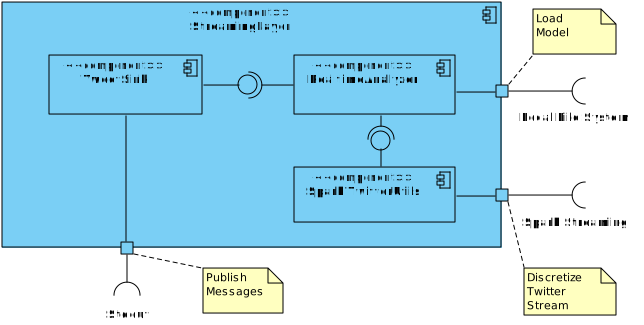
\includegraphics[scale=0.7]{streaming_layer.pdf}
	\caption{Innenansicht der Streaming-Layer Komponente}
	\label{figure:demo_app_streaminglayer}
\end{figure}

In der Komponente RealtimeAnalyzer wurden vor dem Start des Datenstroms Funktionen zur Bewertung einzelner Tweets registriert (VERWEIS?).\\

Die Funktion \lstinline|ScoreTweets| zur Bewertung einzelner Tweets

\[\lstinline|ScoreTweets|: Tweets \longrightarrow \rm I\!R \times Tweets\]
\[tweet \mapsto (score, tweet)\]

wird dabei wie in Listing \ref{lst:tweet_score} dargestellt implementiert:

\begin{lstlisting}[language=Scala,caption={Bewertung von Tweets},label={lst:tweet_score}]
// Split text string into single words
val splitTweets = {
  stream.map(status =>
    (status.getText.split(" "), status)
  )
}

// calculate score for each word, then sum the scores and normalize
val scoredTweets = {
  splitTweets.map(splitTweet => {
    (splitTweet._1.map(word =>
      broadcastScores.value.apply(
         hashingTF.indexOf(word.toLowerCase
           .replaceAll("[^a-zA-Z0-9]", " ")))
     ).sum./(splitTweet._2.getText.split(" ").length),
      splitTweet._2
      )}
  )
}
\end{lstlisting}

Folgendes geschieht Folgendes:
\begin{enumerate}
	\item Extrahieren des Textinhaltes (Metadaten werden ignoriert)
	\item Zerlegen des Textes in einzelne Wörter
	\item Normalisieren der Wörter durch Umwandeln in Kleinbuchstaben und Entfernen von Sonderzeichen
	\item Index der einzelnen Wörter im TF-IDF-Vektor berechnen und dem eingetragenen Score zuweisen (Map)
	\item Scores aller Wörter eines Tweets summieren (Reduce)
	\item Normalisieren des Scores per Division durch die Anzahl aller Wörter des Tweets
	\item Rückgabe des Tupels \textit{(Score, Status)}
\end{enumerate}

Anschließend werden die erzeugten Tupel nach der Größe des erreichten Scores gefiltert und die verbleibenden Status-Texte an den TweetSink weitergegeben.\\

\paragraph{Presentation Layer}\\
\\

\begin{figure}[ht!]
	\centering
  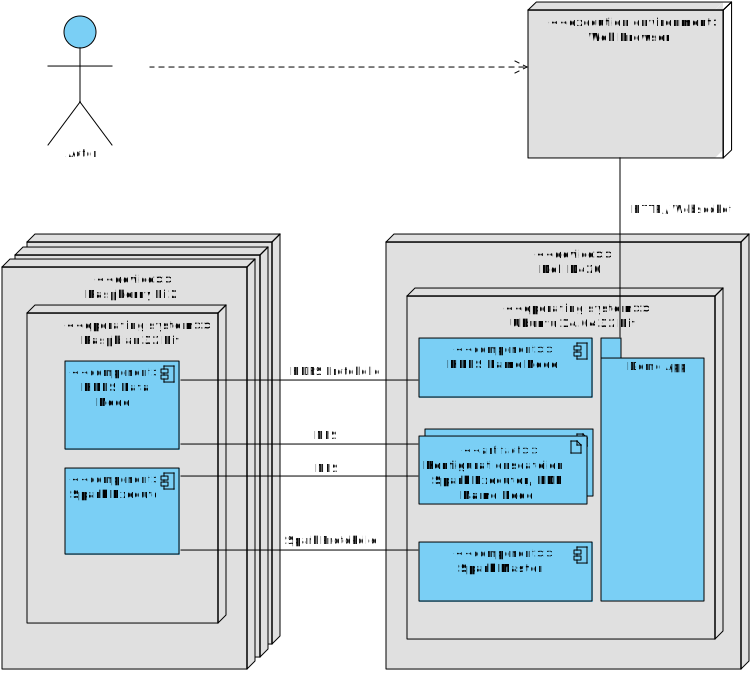
\includegraphics[scale=0.7]{demo_app_deployment.pdf}
	\caption{Verteilungssicht auf die Demo App}
	\label{figure:demo_app_verteilung}
\end{figure}


\begin{figure}[ht!]
	\centering
  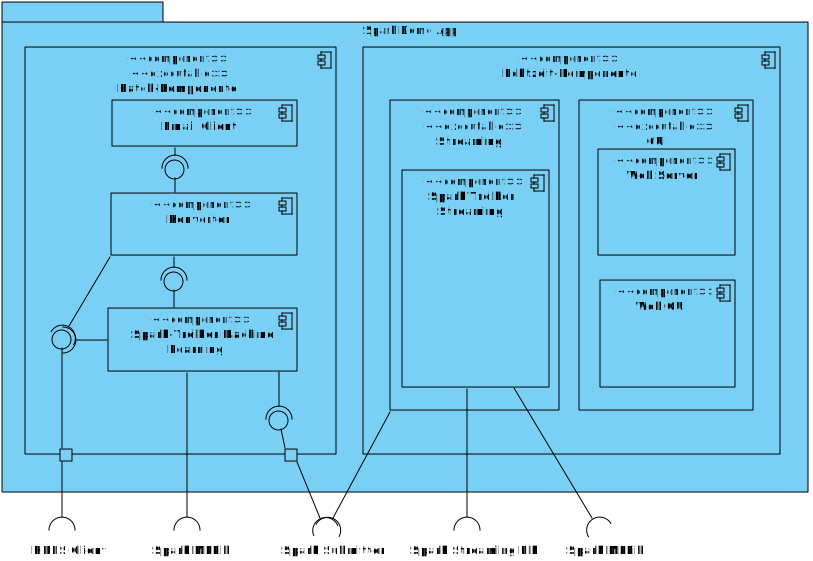
\includegraphics[width=0.9\textwidth]{demo_app_components.pdf}
	\caption{Komponentendiagramm des Demo App Packages}
	\label{figure:demo_app_komponenten}
\end{figure}

\section{Hinweise zur Entwicklung}
Für die Entwicklung hat sich bewährt 

Die Komponenten werden in jeweils eigenen Projekten entwickelt, die sich einzeln auf dem Cluster deployen lassen. Das hat den Vorteil, dass eine einfache Continuous Deployment Pipeline (Abb.~\ref{figure:cd_pipeline}) eingesetzt werden kann, die Änderungen an den jeweiligen Projekten automatisiert auf dem Cluster deployt und so schnellstmögliches Feedback ermöglicht, sowie eine stets lauffähige Codebasis begünstigt.\\

\begin{figure}[ht!]
	\centering
  \includegraphics[scale=0.67]{Pipeline.pdf}
	\caption{Einfache Continuous Deployment Pipeline}
	\label{figure:cd_pipeline}
\end{figure}

Diese Pipeline ist durch ein \textit{post-receive}-Skript in den jeweiligen Repositories der Komponenten auf dem Gateway-Rechner realisiert (Beispiel im Anhang~\ref{subsec:pipeline}).\\


\section{Ergebnisse und Bewertung}

Zur Beurteilung des Laufzeitverhaltens wird die Anwendung in verschiedenen Konfigurationen des Raspberry-Pi-Clusters gestartet. Dabei wird jeweils das Verhalten der einzelnen Komponenten und des gesamten Systems erfasst und zur späteren Auswertung gespeichert.\\

Die zur Laufzeit erfassten Daten sind
\begin{enumerate}
	\item Systemgrößen auf jedem aktiven Knoten (1 Messpunkt pro Sekunde)
	\subitem CPU Nutzung (User, Idle, System, ...)
	\subitem IO Festplatte (Lesen, Schreiben)
	\subitem Swap (Benutzt, Frei)
	\subitem Speicher (Benutzt, Frei, Cached, ...)
	\subitem IO Netzwerk (Gesendet, Empfangen)
	\item Sparkspezifische Größen (1 Messpunkt alle zwei Sekunden)
	\subitem genutzte Cores
	\subitem aktive Stages
	\subitem parallele Receiver (bei Streaming)
	\subitem u.a.\footnote{Bei den sparkspezifischen Messgrößen gibt es viele weitere, die nicht in die Auswertungen einbezogen werden.}
\end{enumerate}

Als Konfigurationsparameter für die Testläufe werden verwendet
\begin{enumerate}
	\item die Blockgröße des Hadoop-Dateisystems HDFS (32MB, 64MB, 128MB)
	\item der Replikationsfaktor der Blöcke auf HDFS (1, 2, 3, 4)
	\item die Anzahl der Worker (1, 2, 4)
\end{enumerate}

Um eine Vergleichbarkeit der Testläufe untereinander zu erreichen werden folgende Größen festgelegt:
\begin{enumerate}
	\item Größe des Textkorpus: 1,5 GB
	\item Fenstergröße des TF-IDF Vektors: 500 Nachrichten
	\item Erlaubte Cores Pro Executor: 4
	\item Erlaubter Arbeitsspeicher pro Executor: 384 MB
	\item Zeitintervall für die Diskretisierung des Datenstroms (Streaming-Komponente): 5 Sekunden
\end{enumerate}

Die \textbf{Größe des Textkorpus} ergibt sich aus der Überlegung eine Datei zu Verarbeiten, die größer als der Arbeitsspeicher eines einzelnen Workers ist, theoretisch aber noch in den geteilten Speicher von vier Executor-Prozessen passt.\\

Die \textbf{Fenstergröße des TF-IDF Vektors} ist willkürlich gewählt. Der Wert 500 entspricht der Anzahl von Email-Nachrichten aus der Spark-User-Mailingliste.\\

Die erlaubten \textbf{Cores pro Executor} entsprechen genau den Verfügbaren Cores auf einem Worker. Damit ist eine volle Ausnutzung der verfügbaren Rechenleistung gewährleistet.\\

Der erlaubte \textbf{Arbeitsspeicher von 384MB pro Executor} lässt bei 1000MB Gesamtspeicher pro Knoten noch Spielraum für das Betriebssystem, den Worker-Prozess und insbesondere den HDFS Data Node für Caching von Dateiblöcken.\\

Das \textbf{Zeitintervall für die Diskretisierung des Datenstroms} richtet sich nach einem Wert, der für den behandelten Anwendungsfall noch als Echtzeit gelten kann.
Ein höherer Wert würde den notwendigen Puffer erhöhen und vermutlich die Verarbeitungszeit pro Datenelement verringern. Ein niedrigerer Wert würde vermutlich den nötigen Puffer verringern und die relative Verarbeitungszeit eines Datenelementes erhöhen. In der folgenden Analyse der Laufzeitverhaltens wird jedoch deutlich, dass der tatsächliche Wert relativ unkritisch für die Stabilität der Komponente ist.\\

Um die Testläufe unter möglichst kontrollierten Bedingungen zu starten, wurde bei jeder Änderung der Konfigurationsparameter das Hadoop-Dateisystem formatiert und der Spark-Cluster zurückgesetzt (inklusive Terminierung und Neustart aller zugehörigen Prozesse).

\subsection{Batch-Komponente}

Die Laufzeitmessung beginnt mit dem Start der ersten Aktion auf einem \gls{RDD} und endet mit der Rückgabe des Relevanzvektors.
Weil die Initialisierung erst zu diesem Zeitpunkt erfolgt, wird der gesamte Prozess von der Kontaktaufnahme zum Cluster und Übermittlung der Tasks bis zur Rückgabe des Ergebnisses gemessen (siehe Listing~\ref{lst:modelbuilder_measuring}).\\

\begin{lstlisting}[language=Scala,caption={Laufzeitmessung},label={lst:modelbuilder_measuring}]
    val documents: RDD[Seq[String]] = sc.textFile(textFile)
      .map(_.toLowerCase)
      .map(_.split(" ").filter(_.length > 2).toSeq)
    val hashingTF = new HashingTF(1 << 20)
    val tf: RDD[Vector] = hashingTF.transform(documents)
    tf.cache() // keep the tf cached because we will be using it twice
		
    val beginFeatureExtraction = System.currentTimeMillis()

    val idf = new IDF().fit(tf) // end stage 0, execution starts here
    val tfidf: RDD[Vector] = idf.transform(tf) // end stage 1

    val relevanceVector = tfidf
      .take(docWindowSize)
      .reduce((vector1, vector2) =>
        addSparseVectors(vector1.asInstanceOf[SparseVector], 
				vector2.asInstanceOf[SparseVector])
      ) // end stage 2, execution ends here

    val finishFeatureExtraction = System.currentTimeMillis()
\end{lstlisting}

Die Zeilen 1-6 in Listing~\ref{lst:modelbuilder_measuring} wurden in die Darstellung aufgenommen, um die Lineage vollständig darzustellen.\\

Der übrige Teil der Anwendung - insbesondere das Abrufen und Prozessieren neu eingegangener Emails - wird nicht berücksichtigt. Bei einem laufenden System sind die dort entstehenden Lasten so gering, dass kein Bedarf für Skalierung besteht.

Tabelle~\ref{table:scaling} zeigt die Laufzeiten der Modelbuilderkomponente bei verschiedenen Konfigurationseinstellungen des Clusters.

\begin{table}[ht]
	\centering % used for centering table
	\begin{tabular}{c c c c} % centered columns (4 columns)
	\hline\hline %inserts double horizontal lines
	Anzahl Worker & Replikationslevel & HDFS Blockgröße (MB) & Laufzeit (Sekunden) \\ [0.5ex] % inserts table
	%heading
	\hline % inserts single horizontal line
	1 & 1 & 32 & 697 \\ % inserting body of the table
	1 & 1 & 64 & 750 \\
	1 & 1 & 128 & 850 (*)\\
	2 & 2 & 32 & 366 \\
	2 & 2 & 64 & 448 \\
	2 & 2 & 128 & 615 \\
	4 & 3 & 32 & 210 \\
	4 & 4 & 32 & 209 (*)\\
	4 & 2 & 64 & 301 \\
	4 & 3 & 64 & 359 \\
	4 & 2 & 128 & 432 \\
	4 & 3 & 128 & 433 \\ [1ex] 
	\hline %inserts single line
	\end{tabular}
	\caption{Skalierungsverhalten des ModelBuilders} % title of Table
	\label{table:scaling} % is used to refer this table in the text
\end{table}

Einen besonderen Einfluss auf die Laufzeit hat offenbar die Blockgröße. Bei gleicher Anzahl von Workern und Replikaten verschlechtert sich die Laufzeit in jedem Versuch bei zunehmender Blockgröße. Diese Beobachtung deckt sich mit den in Tabelle~\ref{table:worker_harddrive} dargestellten Eigenschaften des Festspeichers auf den Workern: 
Im Gegensatz zu den Durchsatzraten der mechanischen Festplatte des Masters verschlechtert sich auf den SD-Karten des Workers der Durchsatz bei zunehmender Blockgröße.\\
Ab einer Blockgröße von 128MB ist es zusätzlich nicht mehr möglich vier Blöcke parallel im Arbeitsspeicher des Executor zu halten (384MB) und diese getrennt auf den 4 verfügbaren Cores verarbeiten zu lassen.

\begin{figure}[ht!]
	\centering
  \includegraphics[width=\textwidth]{runtime_vs_blocksize.pdf}
	\caption{Laufzeit der Feature Extraction bei unterschiedlichen HDFS Blockgrößen}
	\label{figure:runtime_vs_blocksize}
\end{figure}

Ein Hinweis auf den Flaschenhals bei der Verarbeitung auf einem einzigen Knoten ist in Abbildung~\ref{figure:1W32B1R_net_cpu} zu erkennen. Die CPU steht unter Volllast, während die Leistung beim Lesen von der SD-Karte deutlich unter dem idealen Durchsatz bleibt (siehe Tabelle~\ref{table:worker_harddrive}).\\
Netzwerkdurchsatz spielt hier - wie bei einem einzelnen Knoten zu erwarten - offenbar keine Rolle.

\begin{figure}[ht!]
	\centering
  \includegraphics[width=\textwidth]{1W32B1R_net_cpu.pdf}
	\caption{Auslastungskurven bei einem Worker und 32MB Blockgröße}
	\label{figure:1W32B1R_net_cpu}
\end{figure}



\subsection{Echtzeitkomponente}

Eine laufende Anwendung startet auf dem Host des Treibers eine Weboberfläche, die den aktuellen Verlauf des Programms verfolgen lässt. In Abb.~\ref{figure:realtime_dashboard_stats}) sind die dort Lauf mit einem Worker

\begin{figure}[ht!]
	\centering
	\includegraphics[width=0.9\textwidth]{bilder/streaming_stats_dashboard.PNG}
	\caption{Spark-Dashboard des Realtime Analyzers - Statistics}
	\label{figure:realtime_dashboard_stats}
\end{figure}


\subsection{Zusammenfassung}
